\chapter{Application to Market Liquidity}
In this chapter we apply a kernel change point detection algorithm to market data acquired from the Chicago Mercantile Exchange (CME). A short review of related work is covered in section \ref{related_work}. Background on the specific characteristics of data is provided in section \ref{prop_book}, as well as how the datasets are constructed in section \ref{liq_data_construction}. We then summarize the results with exploratory plots and discussion in section \ref{cp_analysis}.

\section{Motivation}
In finance, \textit{market liquidity} describes how quickly a market participant may buy or sell an asset without causing significant fluctuations in the price. In liquid markets, there is minimal impact to the price by quickly buying (selling) it. In illiquid markets, a purchase (sale) of the asset will cause the price to rise (fall) resulting in adverse price selection if the buyer (seller) is making a large transaction. In both cases, market liquidity is in constant fluctuation. By detecting changes in market liquidity a market participant can identify periods of when trading may be more or less favourable. 

One example is a market participant who is particularly sensitive to \textit{market liquidity risk}. Market liquidity risk is the loss incurred when a market participant wishes to execute a trade or eliminate a position while not hitting the
market price \cite{basel2008principles}. The greater the sparsity in a market, the greater the market liquidity risk at the time of trade.  For example, an institutional investor wishing to buy a large position over the course of several days may want to quickly detect low levels in liquidity that could cause them to lift the price inadvertently, resulting in adverse price selection on subsequent executions of their trade. Framing liquidity changes over time as an online change point detection problem is the focus of this chapter. We begin with a broad review of some related studies on market liquidity.

\section{Related Work}
\label{related_work}
A substantial portion of the market liquidity literature focuses on equity markets. For example, market liquidity and trading volume around equity earnings announcements is explored in \cite{kim1994market}. In \cite{chordia2001market}, an aggregate view of market liquidity using transaction data is presented over an eleven year period where the authors found market volatility, short and long term interest rates, the day of the week, and recent market movements were variables that affected market liquidity. Other studies have focused on the how market liquidity changes can be indicative of shifts in market sentiment \cite{baker2004market} \cite{fang2009stock} \cite{debata2018investor}.

Another focus in the literature how market liquidity shocks can affect bond prices. This is especially important when pricing government bonds as they are often used as an indicator for economic health \cite{zaloom2009read}. Countries that have been studied in this context include the U.S. \cite{mccauley2000iv}, Canada \cite{gungor2017has}, Denmark \cite{dick2013funding}, and Japan \cite{sakiyama2016market}. Liquidity risks have also been analysed in the pricing of corporate bond markets as well \cite{de2012liquidity}. Finally, a detailed reference on the subject of optimal execution and how it can impact market liquidity can be found in \cite{gueant2016financial}.

It should be noted that any studies that were done before the new millennium were done before the widespread use of electronic trading platforms. Also, due to the financial crisis between 2007-2008, many new regulations were put into place to reduce systemic risk in the markets. Therefore, any studies prior to these dates may no longer be applicable in the current environment. See  \cite{adrian2017market} and \cite{trebbi2019regulation} for the impacts that U.S. regulations have had on the liquidity of the U.S. fixed income market since 2008.

To our knowledge, no paper has studied intraday changes in market liquidity, especially from a change point detection perspective. While intraday fluctuations are noisy, we believe drastic changes in market liquidity occur at this level of granularity. Before describing the specific datasets, a detailed description of the limit order book is provided based on the notation used in \cite{gould2016queue}. 

\section{Properties of the Limit Order Book}
\label{prop_book}
Many modern financial markets are set-up as an electronic double-sided auction between buyers (bid side) and the sellers (ask side) called \textit{limit order books} (LOBs). A market participant may post orders at specific prices on either side of the book. A limit order, denoted by $x$, is defined as a tuple containing a price, $p_x$, and a size, $w_x$ where $|w_x|>0$:

\begin{equation}
x = \langle p_x, w_x \rangle.
\end{equation}

A limit order's size indicates how many units of an asset a buyer (seller) is willing to trade at $p_x$. The prices for which an order can be submitted at are discrete prices. 

The LOB at time $t$ is denoted as $\mathcal{L}(t)$, and represents the set of all orders currently active at time $t$. All bid orders are at the best bid price or lower. The best bid price at time $t$ is denoted as:
\begin{equation}
\label{top_bid}
b(t) =  \max_{\{x \in \mathcal{L}(t)|w_x<0 \}} p_x.
\end{equation}

All ask orders are placed at the best ask price or higher. The best ask price at a time, $t$, is denoted as:
\begin{equation}
\label{top_ask}
a(t) = \min_{\{x \in \mathcal{L}(t)|w_x>0 \}} p_x.
\end{equation}

The \textit{bid-ask spread} or simply the spread at a time, $t$, is defined as:
\begin{equation}
s(t) = a(t) - b(t)
\end{equation}

The normalized spread, $s_n(t) \geq 0$, can be defined by: 
\begin{equation}
s_n(t) = \frac{s(t)}{\pi} - 1.
\end{equation}

There are many types of orders that can be placed in the LOB. In this context, we assume all orders in the LOB at a given time are basic limit orders. That is, they are orders placed at a specific price with a specific size. Therefore, at a price, $p$, and a time, $t$, the total number of bid orders is:
\begin{equation}
\label{bid_qty}
n^b(p, t) = \sum_{\{x \in \mathcal{L}(t)|w_x<0 , p_x=p\}} |w_x|.
\end{equation}

On the ask side, it is similarly defined as:
\begin{equation}
\label{ask_qty}
n^a(p, t) = \sum_{\{x \in \mathcal{L}(t)|w_x>0 , p_x=p\}}  w_x.
\end{equation}

Everytime a trade occurs or a resting limit order is cancelled or filled at a price, size is removed from the LOB at that price. If the size at the $b(t)$ ($a(t)$) reaches zero then the overall price decreases (increases). It should be obvious then that a lot of pressure on one side or the other can result in large price changes.

Every LOB has a configuration parameter known as the \textit{tick size} denoted by $\pi >0$, which is the smallest possible price increment between two orders at different prices. As mentioned in \cite{gould2016queue}, LOB is essentially a one-dimensional lattice where the dimension is price and every point on the price axis is a multiple\footnote{In most cases these multiples of $\pi$ are strictly positive but in particular markets there may be negative integers of $\pi$, i.e. a price axis with positive and negative prices.} of $\pi$.

The point of interest with this data is detecting how the entire distribution of liquidity changes over time as shown in figure \ref{fig:book_img}. These changes are often associated with events happening in the market such as the start of U.S. trading hours, the release of economic data or a planned speech by the chairman of the federal reserve. There may also be unplanned events that affect the overall liquidity in the book such as a terrorist attack or a virus outbreak like the covid-19 virus in 2020.

%\begin{minipage}{0.96\textwidth}
\begin{center} 
\captionof{figure}[Change in Limit Order Book Liquidity]{The limit order book's liquidity drastically changes from a significant amount of liquidity at time $t_1$  (\textbf{left}) to a low amount of liquidity at time $t_2$ (\textbf{right}). In this case, detecting when the LOB liquidity changes as soon as possible is vital for a market participant that wants to avoid market liquidity risk.} 
\ctikzfig{book_drawdown}
\label{fig:book_img} 
%\medskip
%\tiny
\end{center}
%\end{minipage}

%The second is how the distribution of the bid orders differs from the distribution of the ask orders. Typically, the distribution of liquidity on each side of the book is more or less symmetric. However, there have been studies that have shown times when there is an asymmetry between the two sides. This asymmetry has been shown to correlate to price changes \cite{gould2016queue}. This is equivalent to looking for changes in book imbalance.


\section{Dataset Construction}
\label{liq_data_construction}
While many types of financial instruments trade using a limit order book, this thesis will be focused on futures markets found in the Chicago Mercantile Exchange (CME). The reasoning for this is two-fold. The first, unlike bond markets or currency pair markets, liquidity for many futures products is concentrated on a single exchange. This simplifies analysis of liquidity by not having to aggregate data across several exchanges into a synthetic ladder. The second advantage is, unlike equity markets where stocks and exchange traded funds (ETFs) are traded, there are no dark pools available for the futures markets under consideration in this thesis. Again this simplifies where the liquidity data for an instrument may appear.

The futures that will be used in our dataset are based on a combination of selecting the most traded contracts on the CME and representing different asset classes. They are summarized in the following table:

\begin{center}
\captionof{table}{Summary of Futures Studied}
\begin{tabular}{SSSSSS} \toprule
    {Name} & {Asset Class} & {CME Symbol} & {Tick Size (\$)}\\ \midrule
    {E-mini S\&P 500}  & {Equity} & {ES} & 12.5  \\
    {10 Year T-Notes}  & {Fixed Income}  & {ZN} & 15.625   \\
    {Crude Oil}  & {Commodity}  & {CL} & 10    \\
    {Gold} & {Commodity}  & {GC} & 10   \\
    {Euro FX}  & {FX Currency}  & {6E} & 6.25  \\ \bottomrule
\label{futures}
\end{tabular}
\end{center}

For each future contract in table \ref{futures}, the state of the order book is sampled every $10$ seconds from 7 AM to 4 PM EST between January 6, 2020 and April 22, 2020, excluding days that the CME is closed. At every time step, the quantities of the top $N$ prices are sampled using equations \ref{bid_qty} and \ref{ask_qty}. While all the LOBs analysed here have dozens of price levels of liquidity at any given moment, we focus on the first ten price levels, so $N=10$. To determine the prices at which $n^b$ and $n^a$ are sampled at, we start with the top of the book prices from equations \ref{top_bid} and \ref{top_ask} and   increment them by the tick size to get the prices for each of first ten levels of the LOB at time $t$. This yields prices of $p_i^b=b(t) - i\pi$  and $p_i^a=a(t) + i\pi$ where $i$ is an integer counter $\{i \in  \mathbb{Z}: 0<i<9\}$. These prices can then be used to determine what liquidity is available at each price.  For notational simplicity, we will exclude the $t$ and write the number of quotes at the first ten levels as $n_0^b,...,n_9^b$ for the bid side and  $n_0^a,...,n_9^a$ for the ask side. Therefore, at each time step, the input to the kernel algorithm is a $20$ dimensional tuple of the form:
\begin{equation}
\label{liq_tuple}
\langle n_9^b,...,n_0^b, n_0^a,...,n_9^a \rangle.
\end{equation}
As values of equation \ref{liq_tuple} change over time, the kernel change point statistic changes as well. The idea being that higher values of the kernel statistic will indicate recent changes in the liquidity distribution of the LOB, whereas lower relative values of the kernel statistic indicate the market is more or less at a steady state of liquidity. Using the kernel statistic as signal, the practitioner can then be notified of unexpected activity in the market in real-time so they can react appropriately. %This aim of this structure is to replicate the activity levels of a LOB are most concentrated near the top of the book
%\item Spread normalized by tick size, where spread of zero indicates there is no spread and $s: [0, \mathbb{Z}^+]$, 
%The quantity is the number of quotes posted at each tick increment for $N$ price levels away from the best bid (ask) price.

\section{Change Point Analysis}
\label{cp_analysis}
Unlike the experiments in the previous chapter, we do not have the luxury of knowing when the distribution of liquidity will change for our time series. However, this is a more realistic situation where data is constantly streaming and a decision must be made about whether a change point has occurred. Therefore, we approach this situation mostly as an exploratory exercise for discovering interesting moments when the LOB liquidity has dramatically changed. Rather than use a suite of online change point methods, we will focus on a single method for exploring this dataset, namely the NEWMA algorithm. We will discuss the results of the NEWMA algorithm on each instrument one by one. 

The S\&P futures demonstrated the most consistent behaviour from the algorithm. Because of our chosen time period, we could discern the regime change at 9:30AM EST indicating the US equity trading session had officially opened. This results in the kernel change point statistic rising around this time before coming back down to a lower value for the remainder of the day. This is usually followed up by an afternoon spike near the close of the equity markets around 4:00PM EST.  Market makers often prepare for the day's close by reducing quotes posted in the LOB to not be left with a large unhedged position overnight. An example of this entire cycle is shown in figure \ref{fig:es_typical}. These regime changes can be more or less noticeable depending on how much people are trading on a particular day, which is usually related to the broader macroeconomic context. The market open is the most consistently observable phenomenon while the close does not always cause large shifts in liquidity,  but instead is a gradual tapering from over the course of an hour or two. While detecting the opening and close is not a ground-breaking feat, keep in mind the NEWMA algorithm did this non-parametrically with no knowledge of what the data means. 

\begin{minipage}{0.96\textwidth}
\begin{center} 
\captionof{figure}[ES Liquidity Plots on April 1, 2020]{Liquidity for the CME S\&P 500 future contract is sampled every 10 sec from 7AM to 4PM on April 1, 2020 and plotted at the top five price levels on the bid side (\textbf{top}). For ease of visualization, only the liquidity for the first five price levels on the bid side is shown. The NEWMA kernel change point algorithm is then applied to this data and the resulting kernel statistic is plotted over the same time interval (\textbf{bottom}). The book liquidity is low prior to the 9:30AM open and then exhibits a level shift. It remains at this new level for the course of the day until around 3PM as market participants begin adjusting their positions for the upcoming close.} 
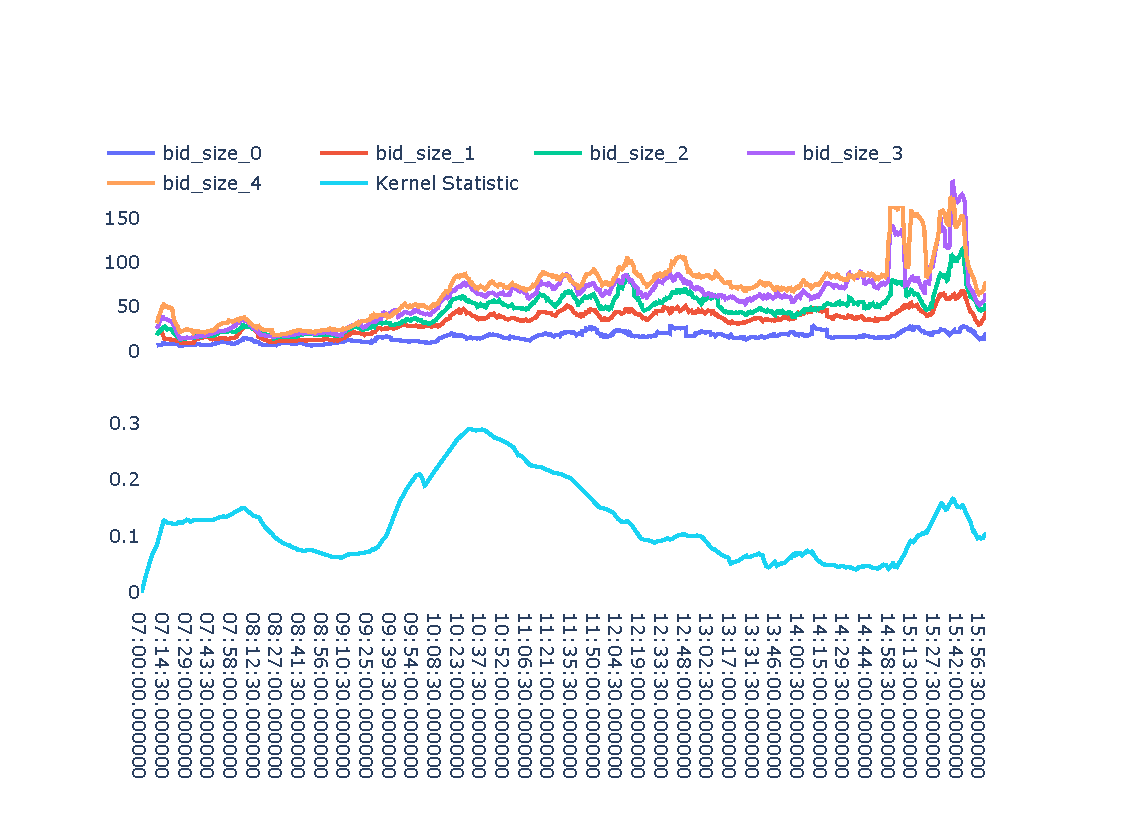
\includegraphics[trim=0cm 1cm 0cm 1cm, clip, width=\textwidth]{es_typical} 
\label{fig:es_typical} 
%\medskip
%\tiny
\end{center}
\end{minipage}

The algorithm did not yield as good results during the month of March 2020. Given the stock market had crashed significantly in early March due to the covid-19 coronavirus \cite{gormsen2020coronavirus}, market liquidity for the S\&P futures was very low for weeks. It is a known phenomenon that when there is a lot of uncertainty, market participants are less willing to trade risky assets such as equities \cite{mccauley2012risk}, resulting in much less liquidity in the market. This results in the liquidity distribution being very close to zero throughout the day, leaving very few chances for a sophisticated, kernel change point algorithm to detect anything. 

Regarding the 10-year U.S. treasury futures, the results were much more mixed and inconsistent. The opening and close were not consistently detected although they should demonstrate similar regime changes during the main U.S. trading hours between 9:30AM and 4PM EST. It is also possible that the 10 sec sampling interval is too often for such a liquid product and a lower sampling rate my lead to reduced noise in the kernel statistic. Finally, there was as significant drop in typical liquidity that was discernible during March that slowly recovered by mid-April though this do not change the performance of the change point detection algorithm on the intraday data. 

The Euro FX future demonstrated some interesting variations in liquidity. Figure \ref{fig:euro_fed_cuts} shows a very drastic imbalance between the two sides of the LOB. We speculate this change in liquidity distribution is a response to the policy changes announced by central banks on that day. The U.S. federal reserve, European central bank, and bank of Japan all announced interest rate cuts and quantitative easing in the wake of the coronavirus pandemic. Another example is shown in figure \ref{fig:euro_bid_fluc} where the bid side liquidity went through some noticeable changes over the course of the day. 

%\begin{minipage}{0.96\textwidth}
\begin{center} 
\captionof{figure}[Euro FX Futures Liquidity Plots on March 16, 2020]{Liquidity for the CME Euro FX future contract is sampled every 10 sec from 7AM to 4PM on March 16, 2020 and plotted at the top five price levels on the bid side (\textbf{top}) and ask side (\textbf{middle}). For ease of visualization, values are only plotted between 9AM and 4PM. The NEWMA kernel change point algorithm is then applied to this data and the resulting kernel statistic is plotted over the same time interval (\textbf{bottom}). }
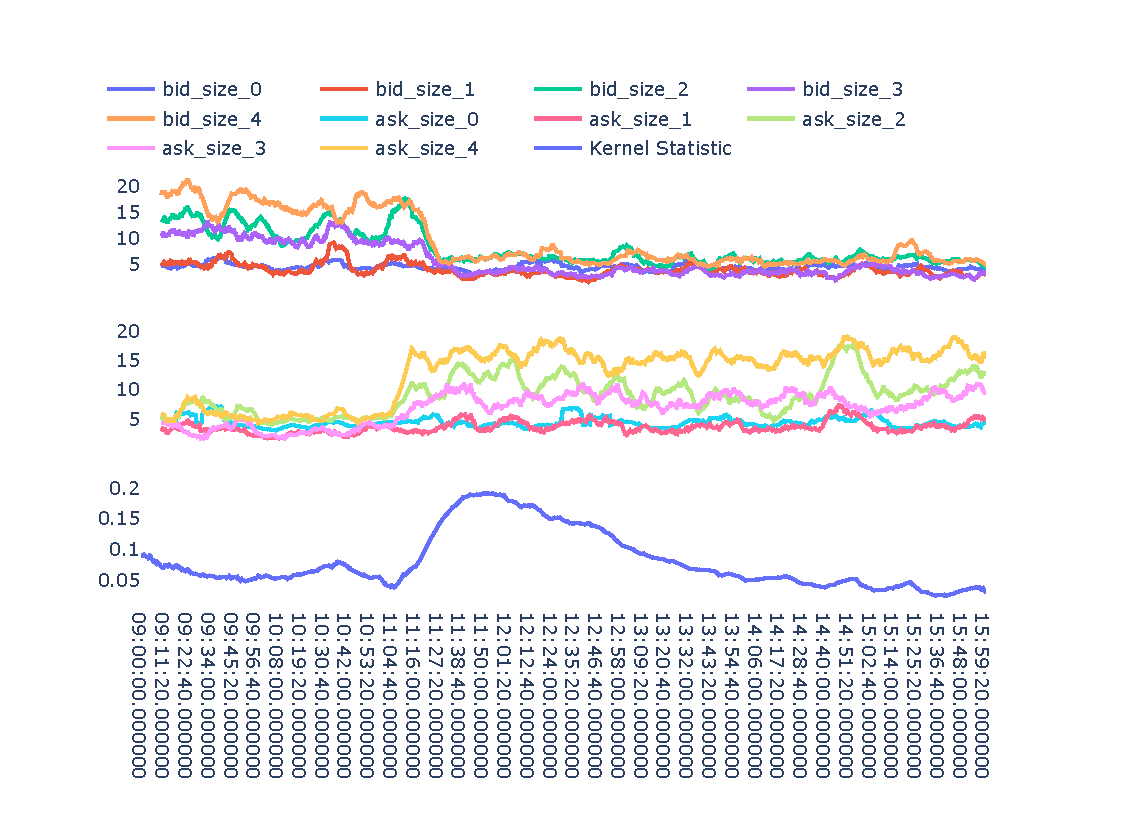
\includegraphics[trim=0cm 1cm 0cm 1cm, clip, width=\textwidth]{euro_fed_cuts} 
\label{fig:euro_fed_cuts} 
%\medskip
%\tiny
\end{center}
%\end{minipage}

%\begin{minipage}{0.96\textwidth}
\begin{center} 
\captionof{figure}[Euro FX Futures Liquidity Plots on March 24, 2020]{Liquidity for the CME Euro FX future contract is sampled every 10 sec from 7AM to 4PM on March 24, 2020 and plotted at the top five price levels on the bid side (\textbf{top}). For ease of visualization, only the liquidity for first five price levels on the bid side is shown between 11AM and 4PM. The NEWMA kernel change point algorithm is then applied to this data and the resulting kernel statistic is plotted over the same time interval (\textbf{bottom}). On this day, several European countries announced stimulus packages, including Italy, Germany and Spain.}
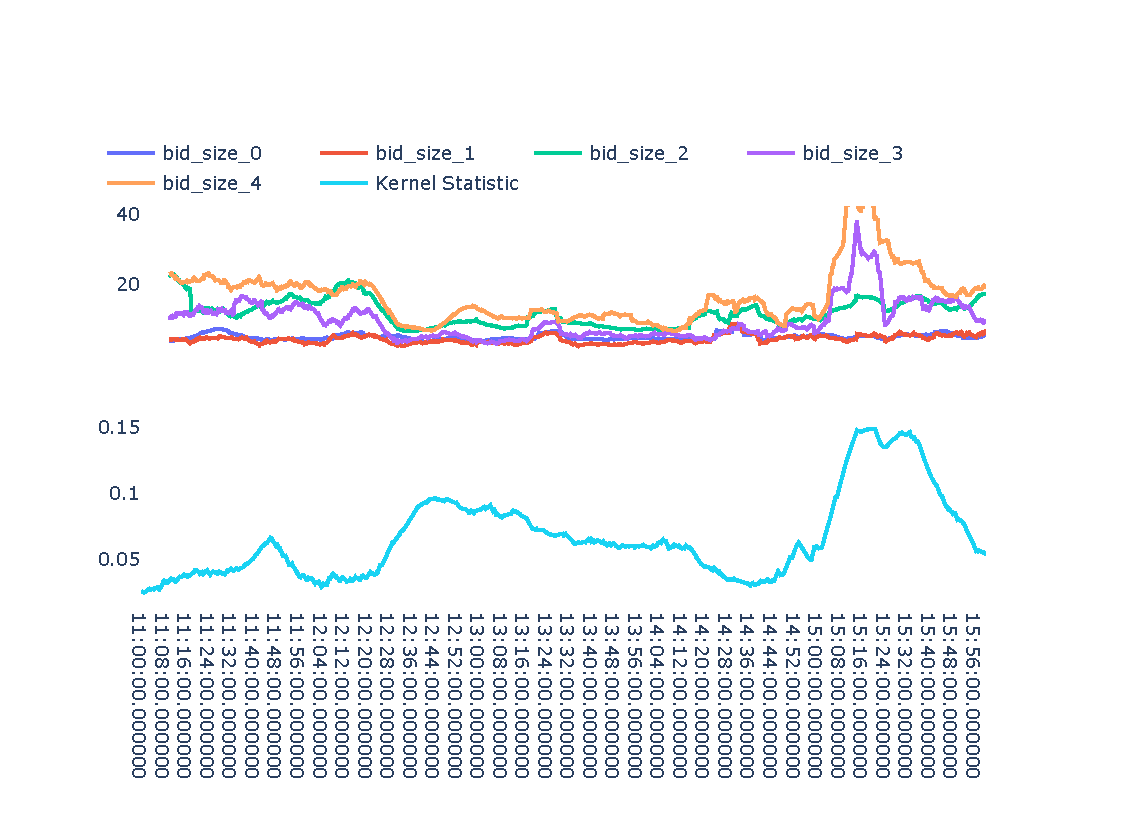
\includegraphics[trim=0cm 1cm 0cm 1cm, clip, width=\textwidth]{euro_bid_change} 
\label{fig:euro_bid_fluc} 
%\medskip
%\tiny
\end{center}
%\end{minipage}

Finally, the two commodity futures, crude oil and gold, exhibited some interesting characteristics. The time period we looked at had especially strange market conditions for both commodities. Gold is known to be used as a safe haven asset during uncertain times \cite{cheema20202008}, so March and April yielded a lot of activity for gold speculation. Figure \ref{fig:gc_fluc} highlights a particular example of a volatile day for market liquidity in gold. Simultaneously, there was an oil pricing war between Russia and Iran that caused an influx of supply into the market to drive down crude oil prices. This combined with little oil and gasoline consumption due to virus shut downs meant crude oil markets were also very turbulent \cite{albulescu2020coronavirus}. Unfortunately, there are no clear-cut examples that we can show for oil. It also worth mentioning that oil prices went negative in April 20, 2020 for the first time ever. Ironically, looking at just the liquidity charts for that day shows an average day in terms of changes and raw sizes. Evaluating market conditions through one lens is not sufficient for understanding the bigger picture.

%\begin{minipage}{0.96\textwidth}
\begin{center} 
\captionof{figure}[Gold Futures Liquidity Plots on March 18, 2020]{Liquidity for the CME gold future contract is sampled every 10 sec from 7AM to 4PM on March 18, 2020 and plotted at the top five price levels on the bid side (\textbf{top}). For ease of visualization, only the liquidity for first five price levels on the bid side is shown. The NEWMA kernel change point algorithm is then applied to this data and the resulting kernel statistic is plotted over the same time interval (\textbf{bottom}). } 
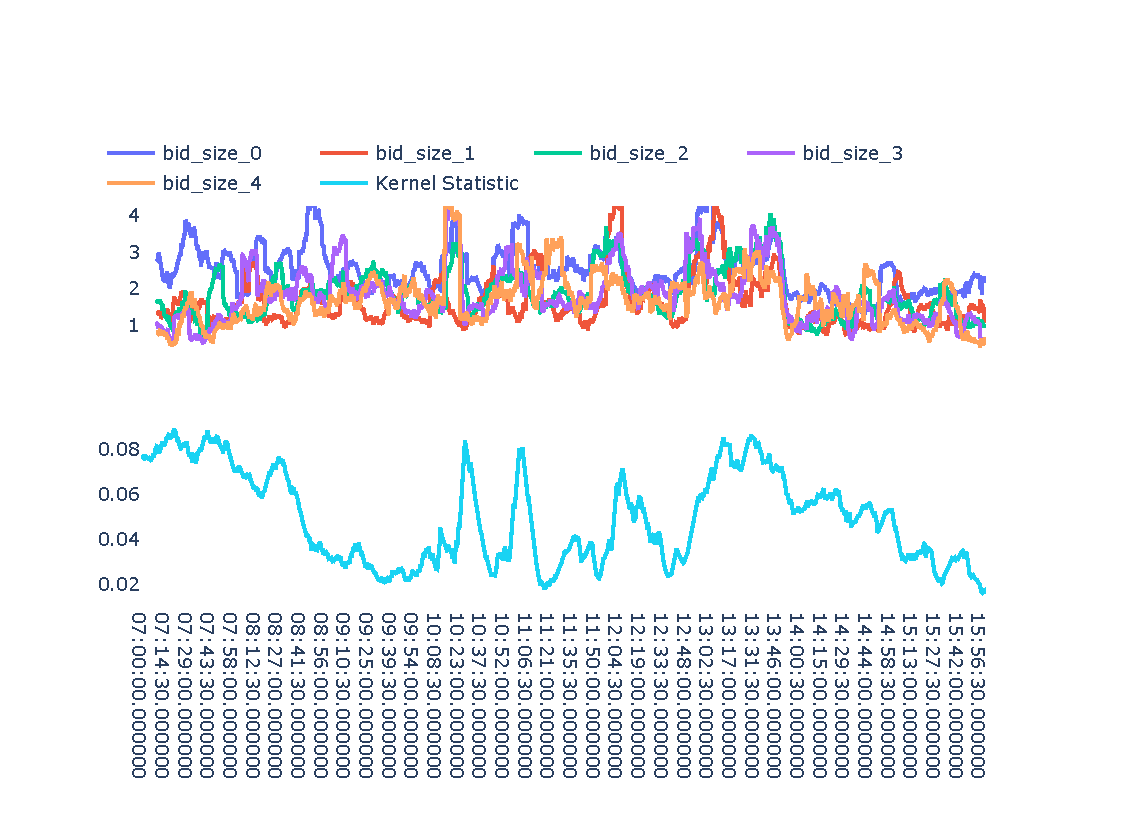
\includegraphics[trim=0cm 1cm 0cm 1cm, clip, width=\textwidth]{gc_fluc} 
\label{fig:gc_fluc} 
%\medskip
%\tiny
\end{center}
%\end{minipage}
